\documentclass[twocolumn, 11pt]{article}

\usepackage{graphicx}
\usepackage{fullpage}
\usepackage{color}

%% \usepackage[condensed]{cabin}
%% \usepackage[T1]{fontenc}
\usepackage{fontspec}
\setmainfont[Ligatures=TeX]{Cabin:series=Condensed}
%\setmainfont[Ligatures=TeX]{Inria}

\usepackage[scale=1,hshift=0,vshift=0,angle=0,opacity=1]{background}

\pagestyle{empty}

\begin{document}
{
  \textcolor{white}{.}\\
  \textcolor{white}{.}\Huge \bf\hspace{0.3em} egnbuevei
}
\backgroundsetup{contents={\includegraphics[width=7.5in,height=10.0in]{title-background}}}

\vspace{1.7em}\noindent
Regnbuevei is a map-building game in which you place tiles to form a rainbow road.  You may play Regnbuevei cooperatively or competitively, and there are a range of scoring options to accommodate a variety of skill levels.

\section*{Objective}

Players will together build a long and beautiful rainbow highway.
Each player will aim to make a particular color (``lane'') the
longest.
\section*{Components}
The game consists of 120 square rainbow tiles, printed on both side with mirror image rainbow portions.

\section*{Setup}

Begin by mixing up the rainbow tiles and forming them into two draw
piles. The draw piles should be located in a draw pile area that can
accommodate a dozen or more draw piles.  Note: because the cards are
double-sided, the top tile in each draw pile will be visible.

Starting with the youngest player, and ending with the oldest player,
players will select a color for their lane of the highway.  The play
will begins with the youngest player and proceed clockwise around the
table.
\begin{figure}[h]
  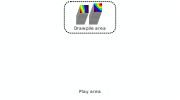
\includegraphics[width=\columnwidth]{draw-piles.png}
  %\caption{The initial setup.}
\end{figure}
\section*{Starting The Game}
The game begins with the first player selecting a tile from the top of
a draw pile and placing it on the play area.  Tiles may not be moved
once placed, so the location and orientation on the play area may
matter.

\section*{The Second Turn And Beyond}
Play continues in a clockwise direction, with each player having two
choices during their turn.  They may either:
\begin{enumerate}
\item draw a tile from the top of a draw pile and play it onto the play area such that it shares at least one edge with a tile that has already played, and that any shared edges match in color,
or
\item split a draw pile by picking up the top half and setting it down
  in the draw pile area.
\end{enumerate}
\begin{figure}[th]
  \includegraphics[width=\columnwidth]{play-example.png}
\end{figure}

\section*{Finishing The Game}
The game ends when one player during their turn is able to play a
tile, and also cannot split a draw pile because all remaining draw
piles consist of just one tile.  See other side for scoring
alternatives.

\section*{Scoring}
There are a number of ways to score the game, and when playing with
very young players it may be wise to use a different scoring rule for
different players.
\subsection*{Prettiest highway}
Players work together to create a beautiful highway.
\subsection*{Longest lane}
The score is the number of tiles forming the longest continuous lane
of the player’s chosen color. The lane may not cross itself, and must
proceed from tile edge to tile edge.  In the following example, the
longest lane for yellow scores 34.

\begin{figure}[h]
  \includegraphics[width=\columnwidth]{scoring-longest.png}
  \caption{Scoring the longest yellow lane gives 35.}
\end{figure}

\subsection*{Largest loop}
The score is for the largest loop of road formed of the player’s
chosen color.

\begin{figure}[h]
  \includegraphics[width=\columnwidth]{scoring-loop.png}
  \caption{Scoring the longest yellow loop gives 16.}
\end{figure}

\backgroundsetup{
  contents={\includegraphics[width=7.5in,height=10.0in]{background}}
}
\subsection*{Team play}
Players may choose to form teams by having several players play with
the same color.  Moreover, players with nearby colors will naturally
assist one another to a certain degree.
\subsection*{Cooperative play}
Scored cooperative play requires the players to decide in advance on
one or more colors to score.  The score is then total distance (either
longest lane or largest loop) for the chosen colors.

\subsection*{A note on colors}
The colors are not all of equal difficulty.  Combined with the
different scoring options, this allows for a range of interesting
handicaps for coping with a wide range of ages and skill levels.

Blue and yellow most flexible, and are recommended for
beginners or for a two-player game between players of similar skill
level.  Green is somewhat more challenging and makes a good third
color for a three-player game.  Purple and red cannot score better
than blue and yellow respectively given the same scoring.  For a
reasonably matched five-player game, we suggest scoring longest loop
for blue and yellow, and longest lane for green, red, and purple.

\section{Legal}
Regnbuevei © 2019 David Roundy. All rights reserved.
\end{document}
